%	PACKAGES AND OTHER DOCUMENT CONFIGURATIONS
%----------------------------------------------------------------------------------

\documentclass[11pt]{article}

\usepackage[top=2cm, bottom=3cm, left=2cm, right=2cm]{geometry}

\setlength{\parindent}{0in}

\newcommand{\Var}{\mathrm{Var}}

\newcommand{\Cov}{\mathrm{Cov}}

\newcommand{\plim}{\rightarrow_{p}}

\usepackage{pdfpages}
\usepackage{amsmath, amsfonts}
\usepackage{graphicx}
\usepackage{bm}
\usepackage{listings}
\usepackage{multirow,array}
\usepackage{enumerate}
\usepackage{bbm}


\usepackage[latin1]{inputenc}

\usepackage{amssymb}
\usepackage{subfig}
\usepackage{mathrsfs}
\usepackage{float}
\usepackage{booktabs}
\usepackage{color}
\usepackage{rotating}
\usepackage{amsthm}
\usepackage{multirow,array}
\usepackage{caption}
\usepackage{url}


\DeclareMathOperator*{\argmax}{arg\,max}
\DeclareMathOperator*{\argmin}{arg\,min}



% Expectation symbol
\newcommand{\E}{\mathrm{E}}
\newcommand{\V}{\mathrm{V}}
\newcommand{\N}{\mathcal{N}}
\newcommand{\R}{\mathbb{R}} 

%----------------------------------------------------------------------------------
%	TITLE AND AUTHOR(S)
%----------------------------------------------------------------------------------
\title{Econ 675 Assignment 6} % The article title


\author{Nathan Mather\thanks{Shouts out to Ani for the help with question 1 }}  % The article author(s) 

\date{\today} % An optional date to appear under the author(s)


%----------------------------------------------------------------------------------
\begin{document}
	
%------------------------------------------------------------------------------
%	TABLE OF CONTENTS & LISTS OF FIGURES AND TABLES
%------------------------------------------------------------------------------
\maketitle % Print the title/author/date block

\setcounter{tocdepth}{2} % Set the depth of the table of contents to show sections and subsections only

\tableofcontents % Print the table of contents


%-------------------------------------------------------------
% Question 1 
%-------------------------------------------------------------

\section{Q1}

TO DO
%-------------------------------------------------------------
% Question 2 
%-------------------------------------------------------------

\section{Question 2: The Effect of Head Start on Child Mortality}

\subsection{Q2.1 RD Plots and Falsification Tests}

\subsubsection{Q2.1.1}

\begin{figure}[H]
	\centering
	\subfloat{
		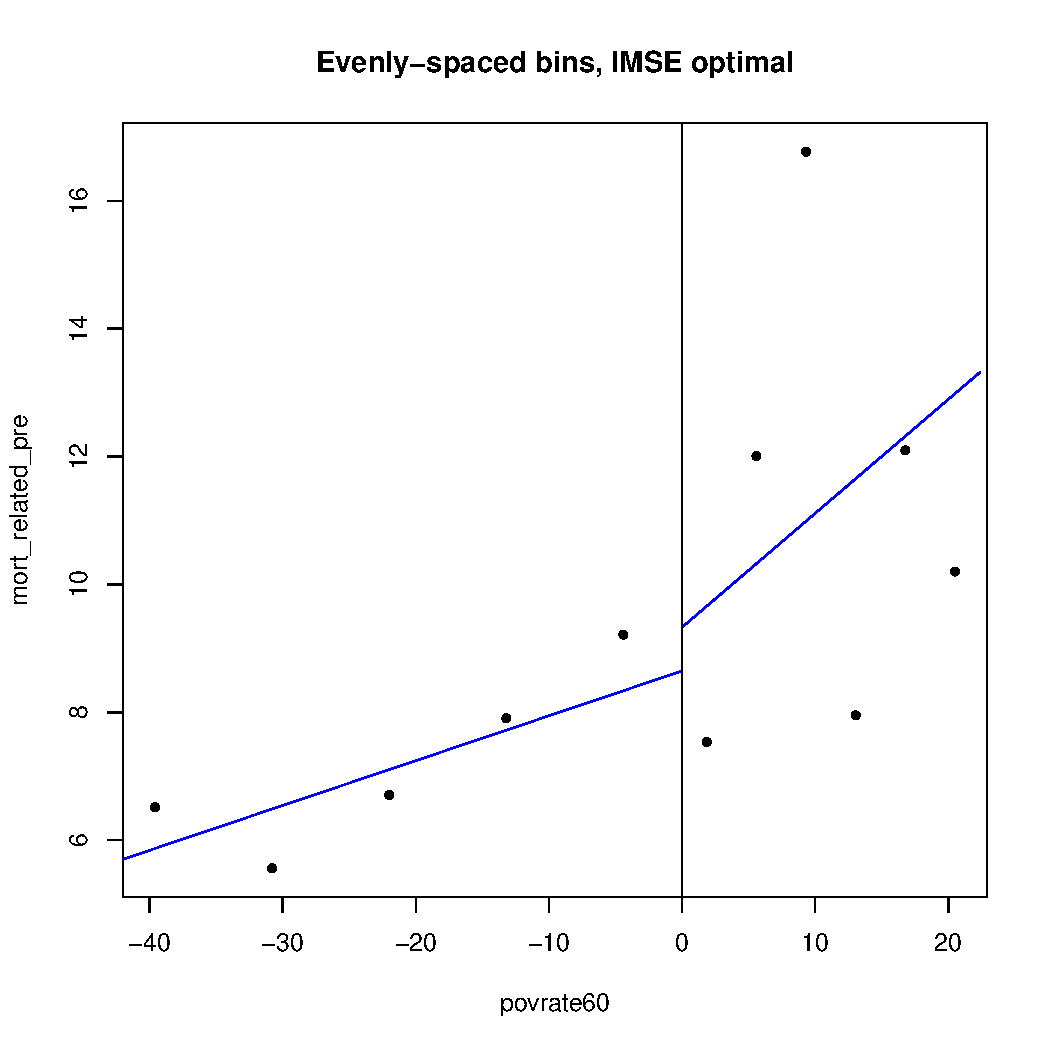
\includegraphics[width=80mm]{plot_211ia.pdf}
	}
	\subfloat{
		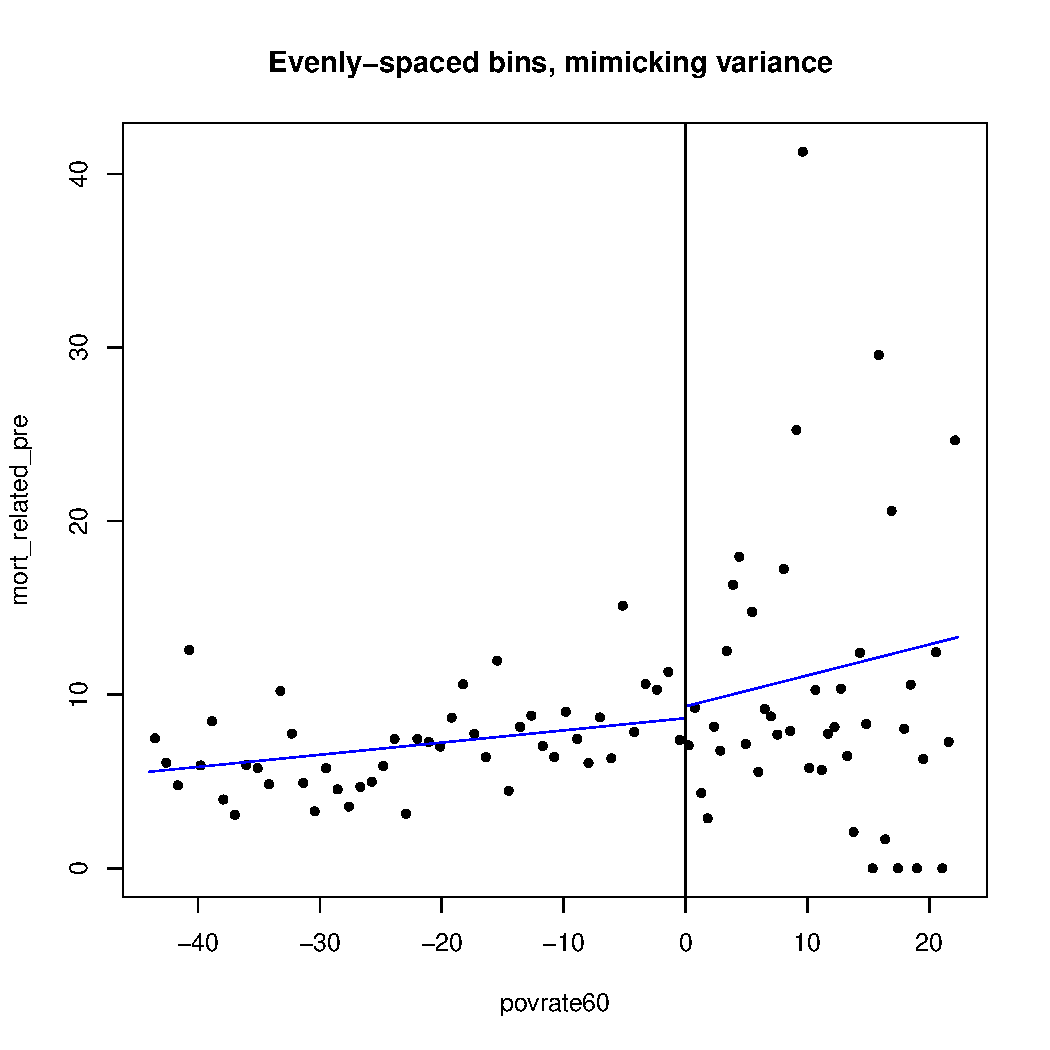
\includegraphics[width=80mm]{plot_211ib.pdf}
	}
	\newline
	\subfloat{
		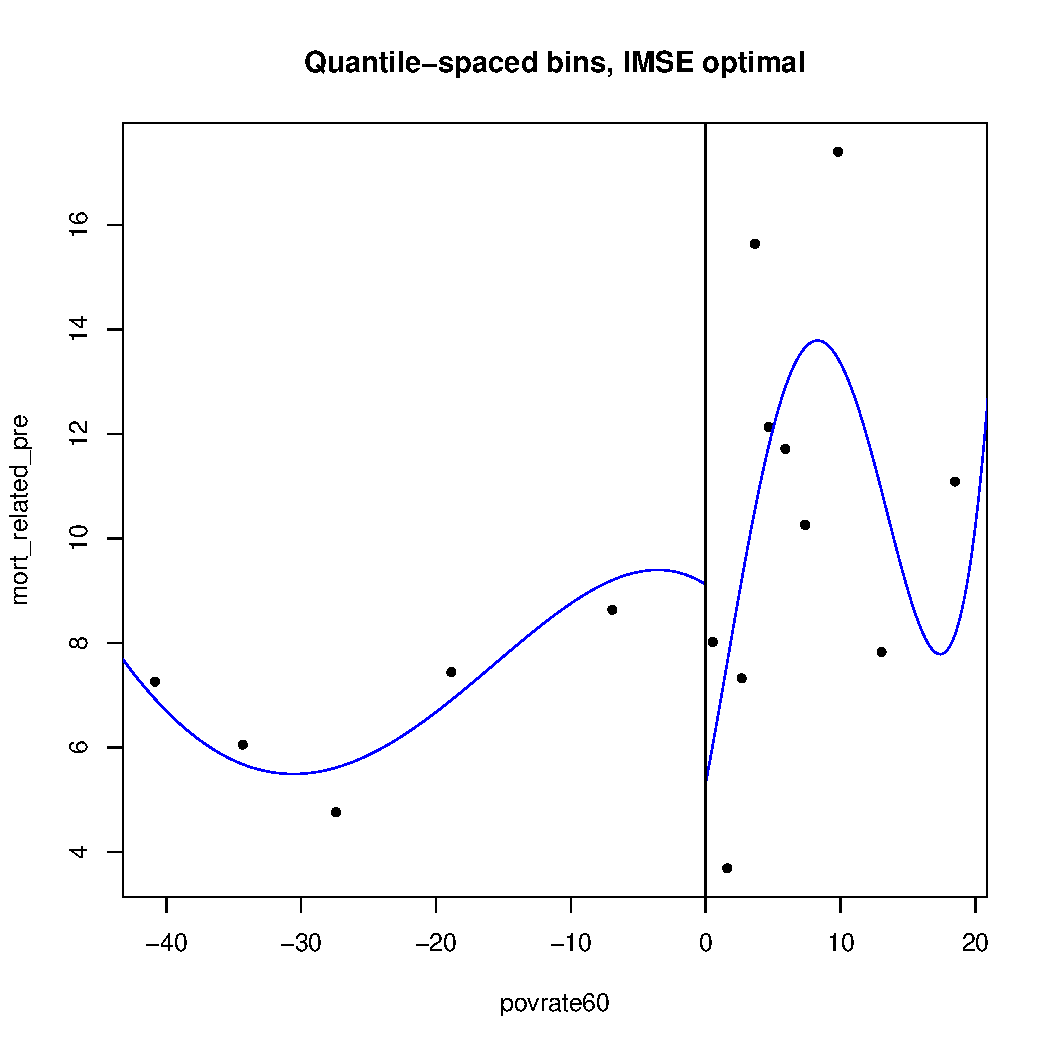
\includegraphics[width=80mm]{plot_211iia.pdf}
	}
	\subfloat{
		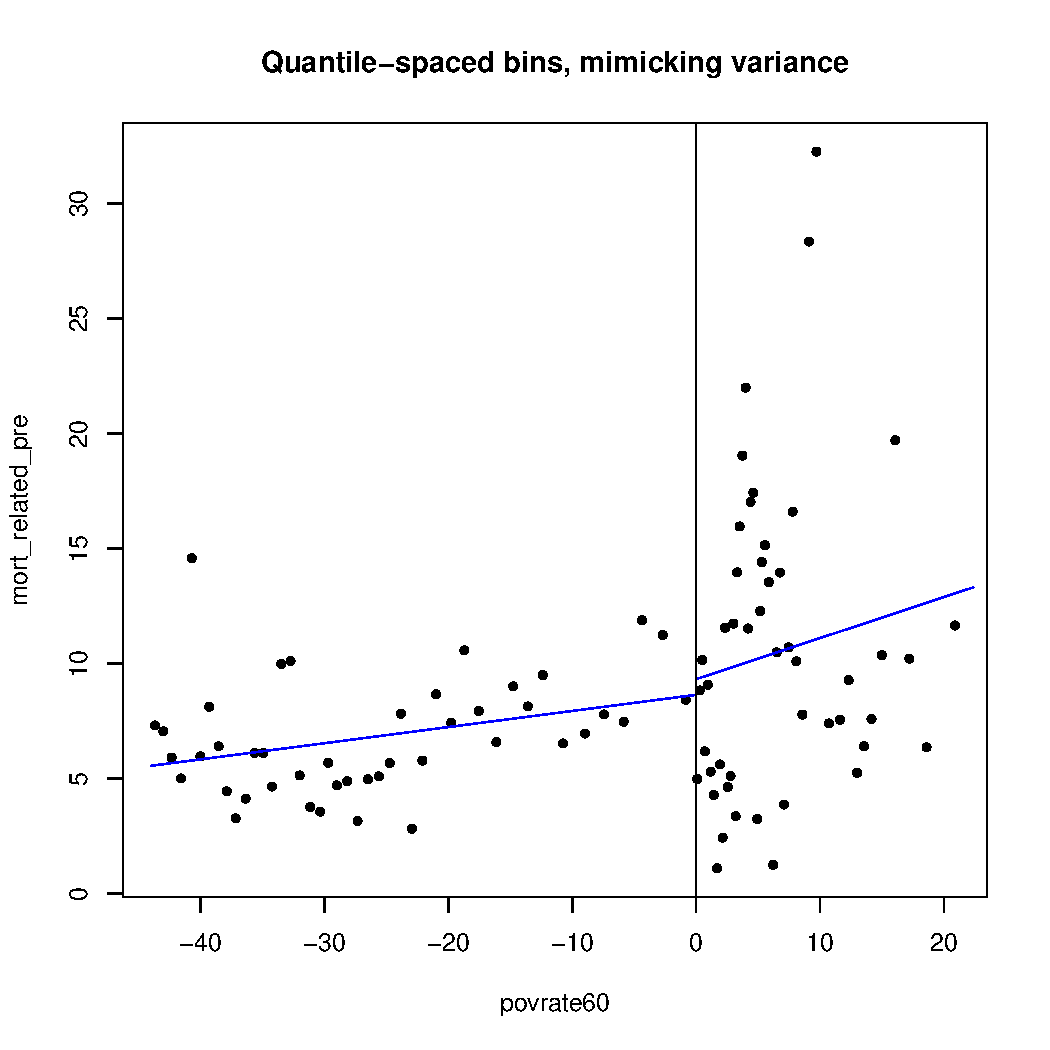
\includegraphics[width=80mm]{plot_211iib.pdf}
	}
	
\end{figure}

\subsubsection{Q2.1.2}
\begin{center}
	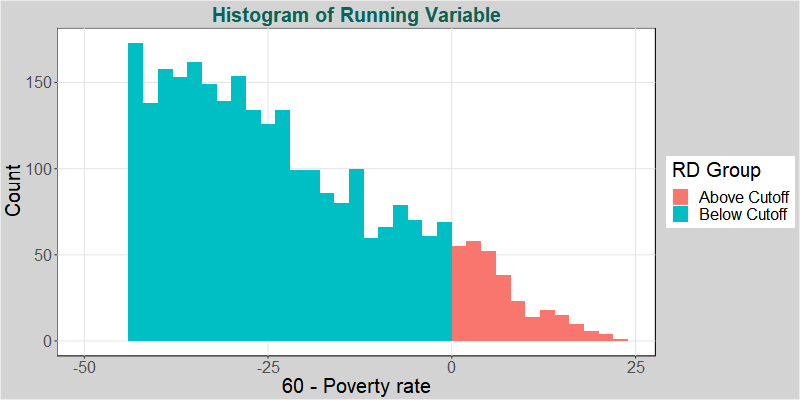
\includegraphics[width=.8\linewidth]{plot_212i.png}
	
\end{center}
\begin{center}
	\centering
	\textbf{local binomial test}\par\medskip
	\scalebox{0.85}{
		% latex table generated in R 3.5.1 by xtable 1.8-3 package
% Sun Dec 09 13:28:06 2018
\begin{tabular}{rrrr}
  \hline
Bandwidth & Number Below Cutoff & Number Above Cutoff & binomial P Valu \\ 
  \hline
0.40 &   6 &   8 & 0.79 \\ 
  0.60 &   9 &  10 & 1.00 \\ 
  0.80 &  12 &  12 & 1.00 \\ 
  1.00 &  18 &  16 & 0.86 \\ 
  1.20 &  20 &  20 & 1.00 \\ 
  1.40 &  24 &  22 & 0.88 \\ 
  1.60 &  28 &  24 & 0.68 \\ 
  1.80 &  32 &  27 & 0.60 \\ 
  2.00 &  35 &  29 & 0.53 \\ 
  2.20 &  43 &  33 & 0.30 \\ 
  2.40 &  44 &  35 & 0.37 \\ 
  2.60 &  51 &  38 & 0.20 \\ 
  2.80 &  53 &  40 & 0.21 \\ 
  3.00 &  53 &  40 & 0.21 \\ 
  3.20 &  54 &  45 & 0.42 \\ 
  3.40 &  58 &  47 & 0.33 \\ 
  3.60 &  62 &  49 & 0.25 \\ 
  3.80 &  64 &  51 & 0.26 \\ 
  4.00 &  69 &  55 & 0.24 \\ 
   \hline
\end{tabular}

	}
\end{center}


\subsection{Q2.2 Global and Flexible Parametric Methods}
\subsubsection{Q2.2.1}

\begin{center}
	\centering
	\textbf{global polynomial fit}\par\medskip
	\scalebox{1}{
		% latex table generated in R 3.5.1 by xtable 1.8-3 package
% Sat Dec 08 21:31:02 2018
\begin{tabular}{lrrrr}
  \hline
value & Polynomial 3 & Polynomial 4 & Polynomial 5 & Polynomial 6 \\ 
  \hline
Estimate & -1.12 & -1.02 & -1.66 & -1.75 \\ 
  Standard Error & 0.67 & 0.76 & 0.86 & 0.87 \\ 
   \hline
\end{tabular}

	}
\end{center}
 .
\\ \\


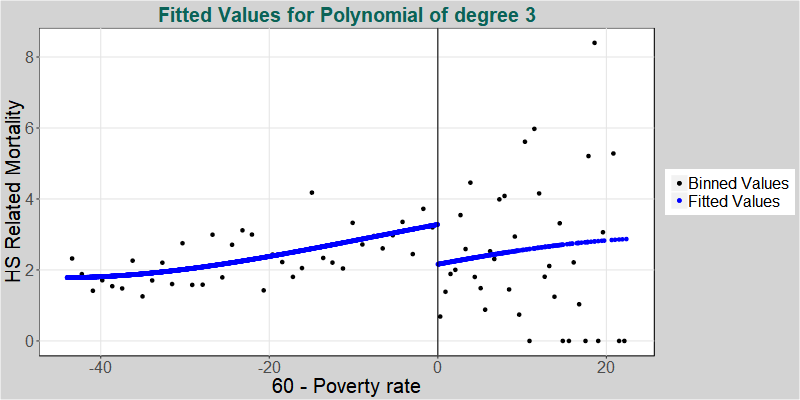
\includegraphics[width=.8\linewidth]{plot_221_poly_3.png}
\\ \\
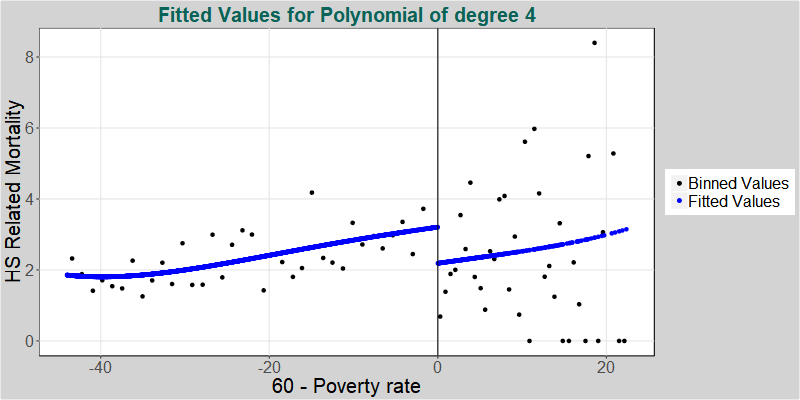
\includegraphics[width=.8\linewidth]{plot_221_poly_4.png}
\\ \\
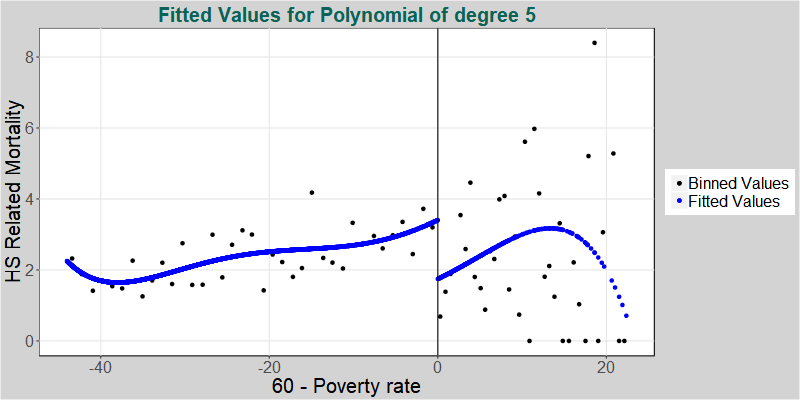
\includegraphics[width=.8\linewidth]{plot_221_poly_5.png}
\\ \\
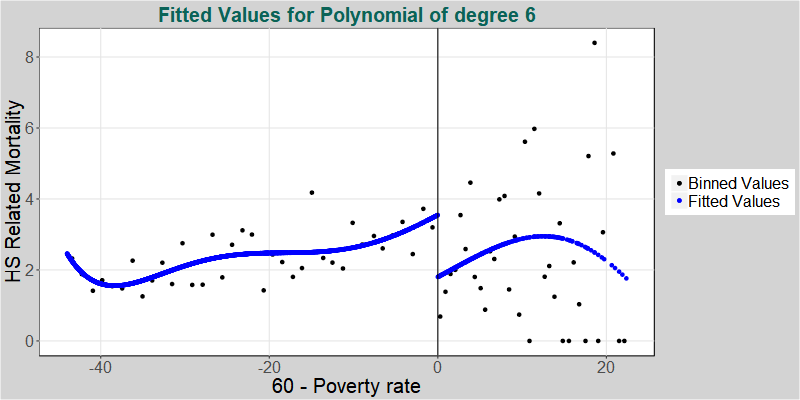
\includegraphics[width=.8\linewidth]{plot_221_poly_6.png}


\subsubsection{Q2.2.2}


\begin{center}
	\centering
	\textbf{global polynomial fit, Fully Interacted }\par\medskip
	\scalebox{1}{
		% latex table generated in R 3.5.1 by xtable 1.8-3 package
% Sat Dec 08 21:31:02 2018
\begin{tabular}{lrrrr}
  \hline
value & Polynomial 3 & Polynomial 4 & Polynomial 5 & Polynomial 6 \\ 
  \hline
Estimate & -2.94 & -10.70 & -45.72 & 28.77 \\ 
  Standard Error & 2.14 & 9.39 & 53.29 & 320.06 \\ 
   \hline
\end{tabular}

	}
\end{center}
 .
\\ \\ 

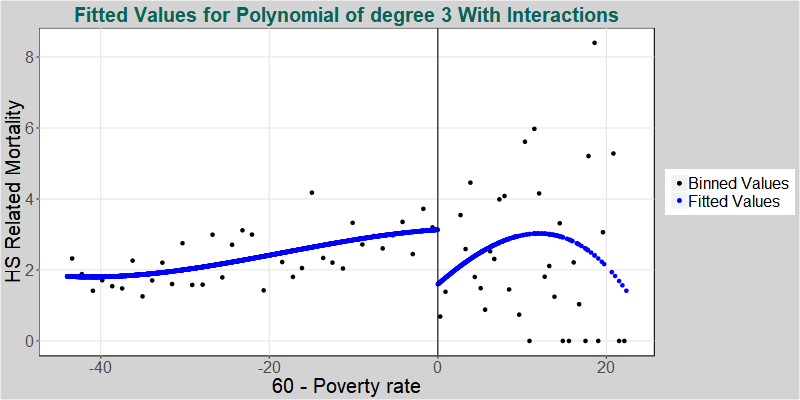
\includegraphics[width=.8\linewidth]{plot_222_poly_3.png}
\\ \\
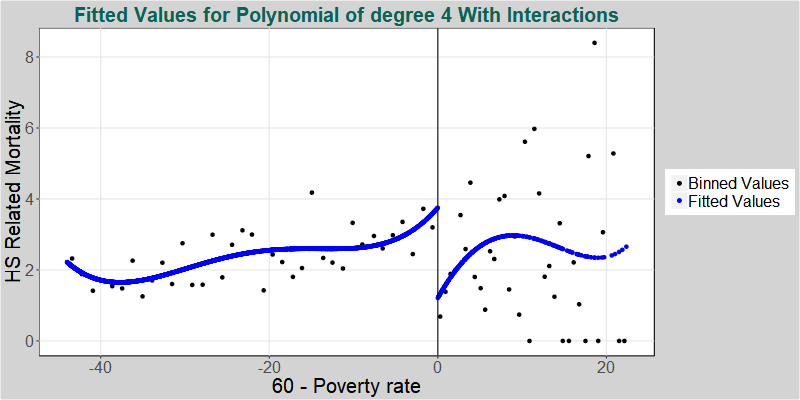
\includegraphics[width=.8\linewidth]{plot_222_poly_4.png}
\\ \\
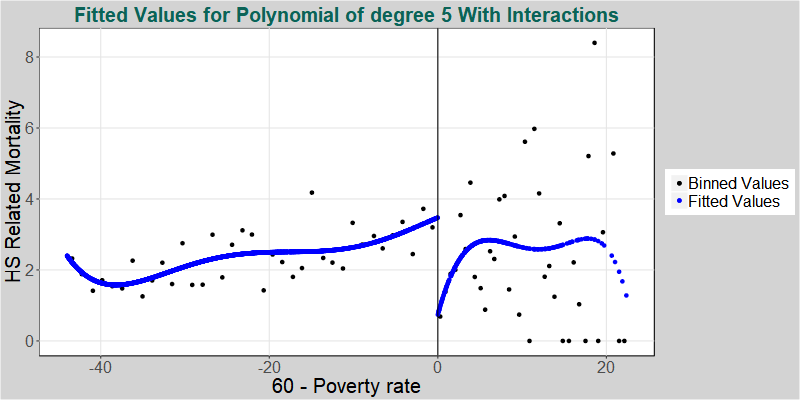
\includegraphics[width=.8\linewidth]{plot_222_poly_5.png}
\\ \\
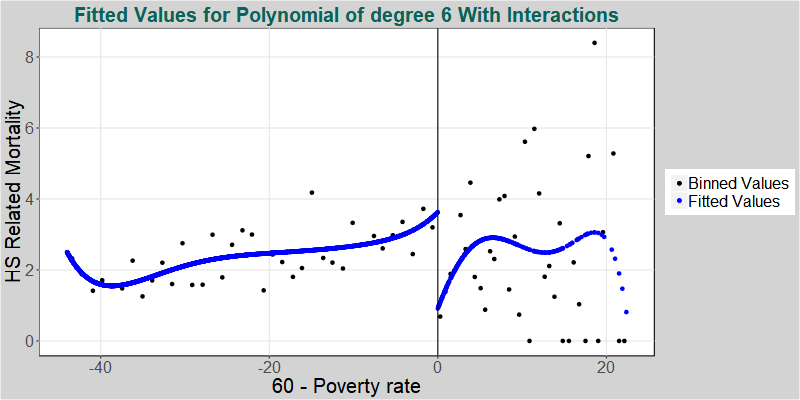
\includegraphics[width=.8\linewidth]{plot_222_poly_6.png}


\subsubsection{Q2.2.3}

% bw 1 
\begin{center}
	\centering
	\textbf{Local Parametric Model Bandwidth of 1 }\par\medskip
	\scalebox{1}{
		% latex table generated in R 3.5.1 by xtable 1.8-3 package
% Sun Dec 09 13:28:12 2018
\begin{tabular}{lrrr}
  \hline
value & Polynomial 1 & Polynomial 2 & Polynomial 3 \\ 
  \hline
Estimate & -2.56 & -2.60 & -5.55 \\ 
  Standard Error & 1.92 & 1.93 & 2.55 \\ 
   \hline
\end{tabular}

	}
\end{center}

\begin{center}
	{\large \bf{Graphs for Bandwidth of 1}}
\end{center}

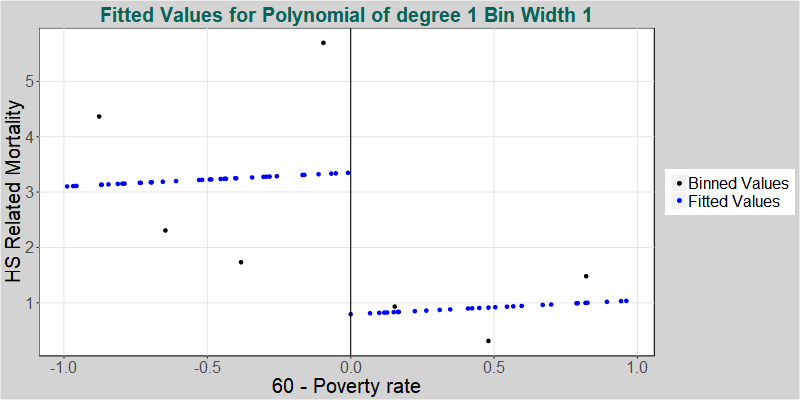
\includegraphics[width=.8\linewidth]{plot_223_poly_1_bw_1.png}
\\ \\
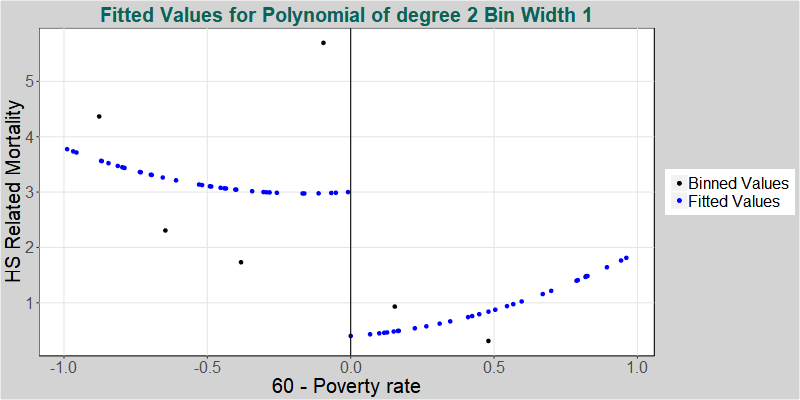
\includegraphics[width=.8\linewidth]{plot_223_poly_2_bw_1.png}
\\ \\
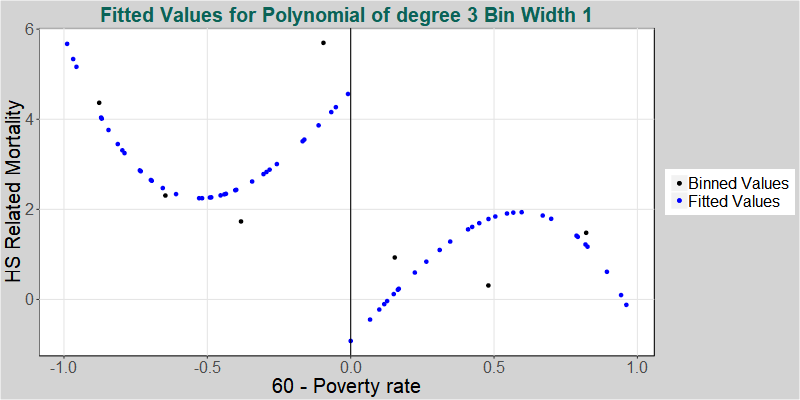
\includegraphics[width=.8\linewidth]{plot_223_poly_3_bw_1.png}

% bw 5 

\begin{center}
	\centering
	\textbf{Local Parametric Model Bandwidth of 5 }\par\medskip
	\scalebox{1}{
		% latex table generated in R 3.5.1 by xtable 1.8-3 package
% Sun Dec 09 13:28:12 2018
\begin{tabular}{lrrr}
  \hline
value & Polynomial 1 & Polynomial 2 & Polynomial 3 \\ 
  \hline
Estimate & -2.26 & -2.40 & -3.92 \\ 
  Standard Error & 1.31 & 1.32 & 1.72 \\ 
   \hline
\end{tabular}

	}
\end{center}

\begin{center}
	{\large \bf{Graphs for Bandwidth of 5}}
\end{center}

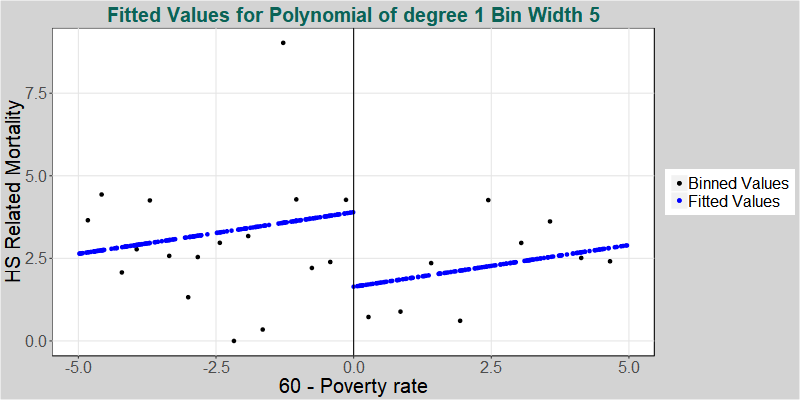
\includegraphics[width=.8\linewidth]{plot_223_poly_1_bw_5.png}
\\ \\
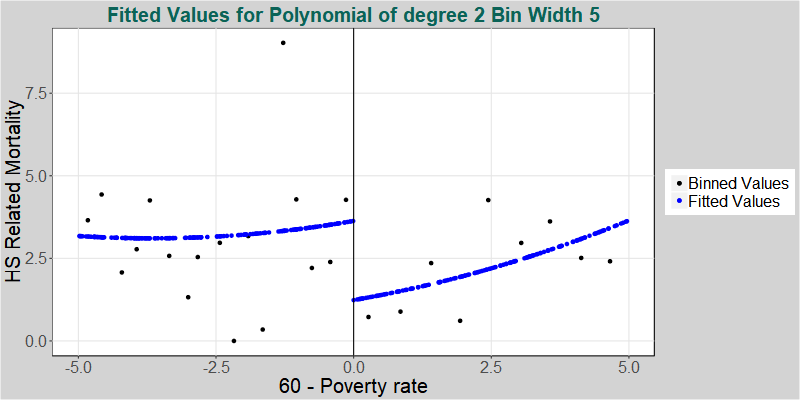
\includegraphics[width=.8\linewidth]{plot_223_poly_2_bw_5.png}
\\ \\
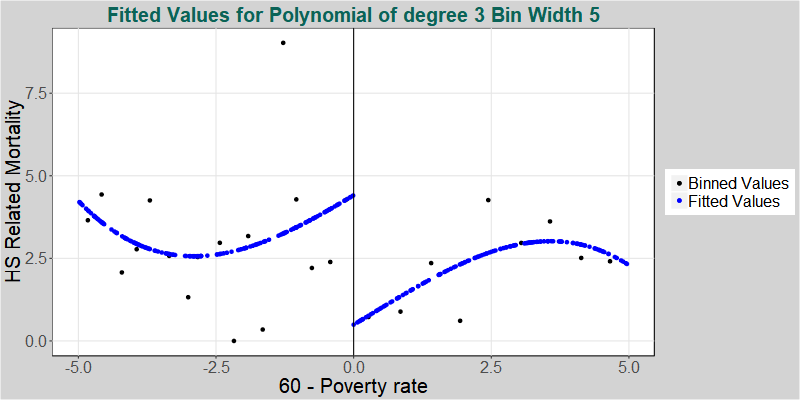
\includegraphics[width=.8\linewidth]{plot_223_poly_3_bw_5.png}


% bw 9 

\begin{center}
	\centering
	\textbf{Local Parametric Model Bandwidth of 9 }\par\medskip
	\scalebox{1}{
		% latex table generated in R 3.5.1 by xtable 1.8-3 package
% Sun Dec 09 13:28:12 2018
\begin{tabular}{lrrr}
  \hline
value & Polynomial 1 & Polynomial 2 & Polynomial 3 \\ 
  \hline
Estimate & -1.84 & -1.89 & -2.28 \\ 
  Standard Error & 0.93 & 0.94 & 1.22 \\ 
   \hline
\end{tabular}

	}
\end{center}

\begin{center}
	{\large \bf{Graphs for Bandwidth of 9}}
\end{center}

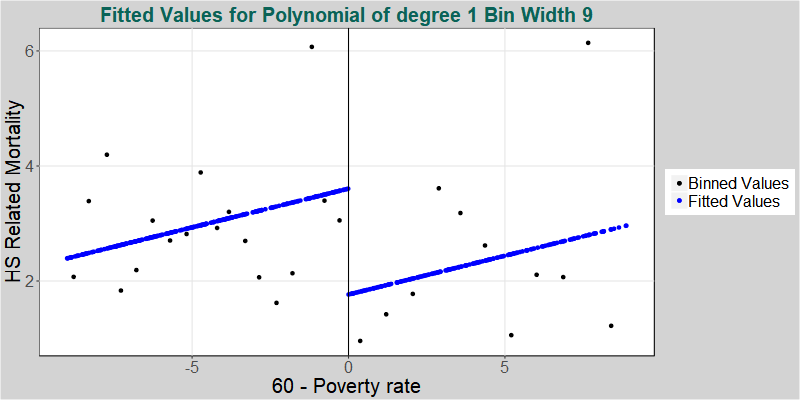
\includegraphics[width=.8\linewidth]{plot_223_poly_1_bw_9.png}
\\ \\
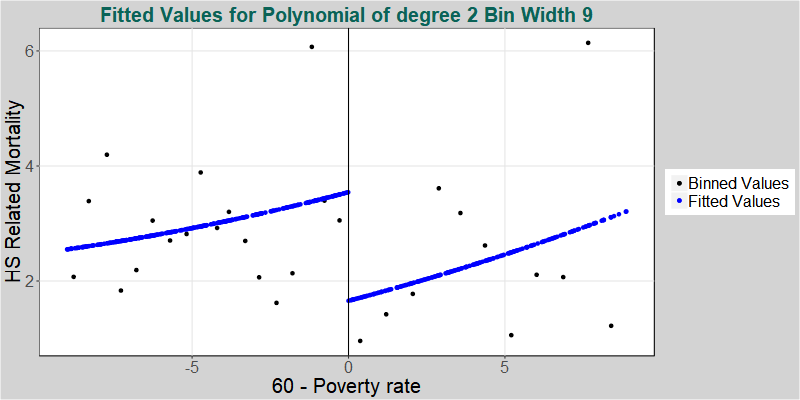
\includegraphics[width=.8\linewidth]{plot_223_poly_2_bw_9.png}
\\ \\
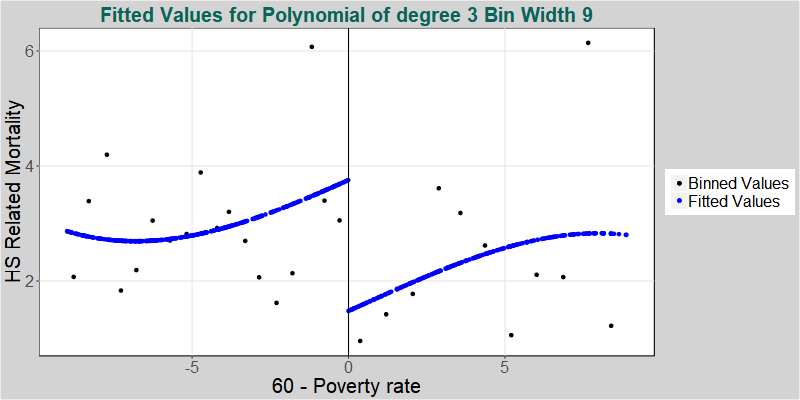
\includegraphics[width=.8\linewidth]{plot_223_poly_3_bw_9.png}
.
\\
\\
% bw 18

\begin{center}
	\centering
	\textbf{Local Parametric Model Bandwidth of 18 }\par\medskip
	\scalebox{1}{
		% latex table generated in R 3.5.1 by xtable 1.8-3 package
% Sun Dec 09 13:28:12 2018
\begin{tabular}{lrrr}
  \hline
value & Polynomial 1 & Polynomial 2 & Polynomial 3 \\ 
  \hline
Estimate & -1.17 & -1.18 & -1.67 \\ 
  Standard Error & 0.76 & 0.80 & 1.02 \\ 
   \hline
\end{tabular}

	}
\end{center}

\begin{center}
	{\large \bf{Graphs for Bandwidth of 18}}
\end{center}

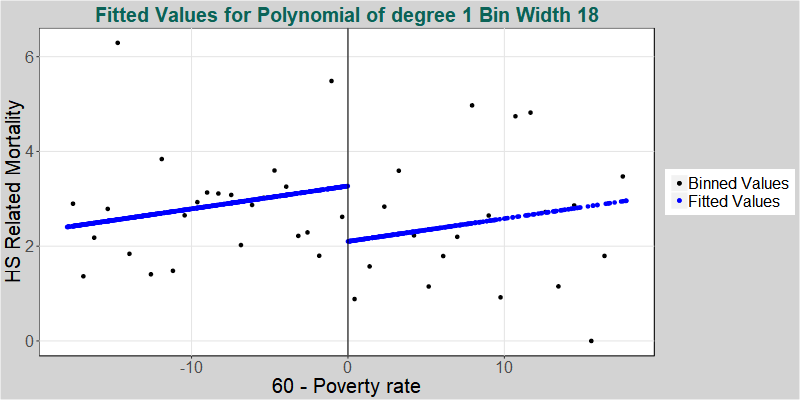
\includegraphics[width=.8\linewidth]{plot_223_poly_1_bw_18.png}
\\ \\
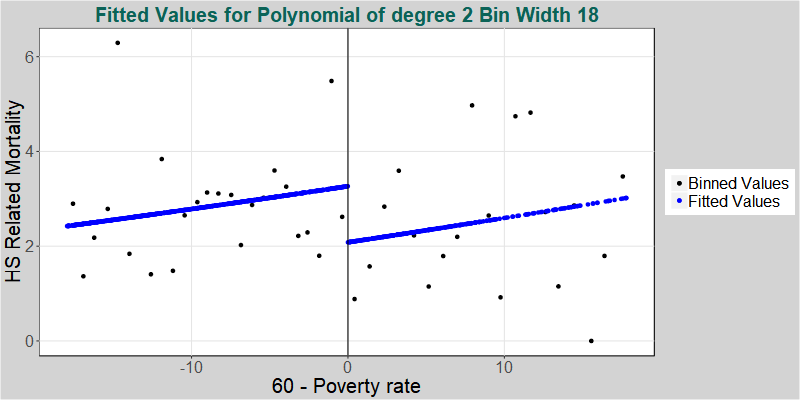
\includegraphics[width=.8\linewidth]{plot_223_poly_2_bw_18.png}
\\ \\
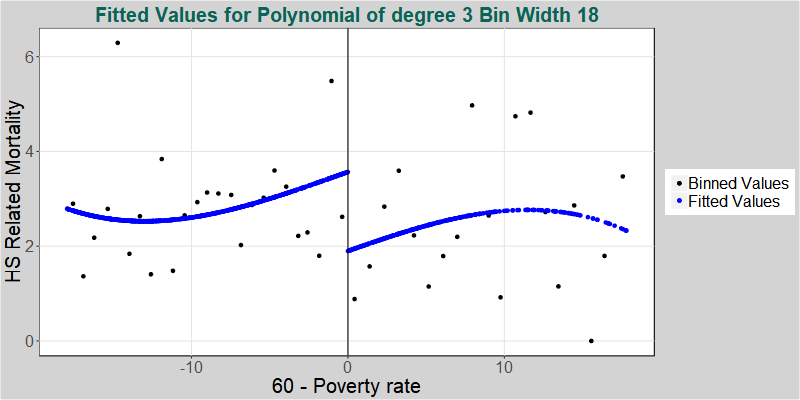
\includegraphics[width=.8\linewidth]{plot_223_poly_3_bw_18.png}

\subsubsection{Q2.2.4}



\subsection{Q2.3 Robust Local Polynomial Methods}

\subsubsection{Q2.3.1}

% poly 0 
\begin{center}
	\centering
	\textbf{Robust local polynomial degree 0  }\par\medskip
	\scalebox{1}{
		% latex table generated in R 3.5.1 by xtable 1.8-3 package
% Sun Dec 09 13:28:13 2018
\begin{tabular}{lrrrrr}
  \hline
Estimator & Coeff & Std. Err. & CI Lower & CI Upper & polynomial \\ 
  \hline
Conventional & -2.11 & 0.99 & -4.05 & -0.17 &   0 \\ 
  Bias-Corrected & -2.56 & 0.99 & -4.50 & -0.62 &   0 \\ 
  Robust & -2.56 & 1.23 & -4.96 & -0.15 &   0 \\ 
   \hline
\end{tabular}

	}
\end{center}

% poly 1
\begin{center}
	\centering
	\textbf{Robust local polynomial degree 1  }\par\medskip
	\scalebox{1}{
		% latex table generated in R 3.5.1 by xtable 1.8-3 package
% Sun Dec 09 13:28:13 2018
\begin{tabular}{lrrrrr}
  \hline
Estimator & Coeff & Std. Err. & CI Lower & CI Upper & polynomial \\ 
  \hline
Conventional & -2.41 & 1.21 & -4.77 & -0.05 &   1 \\ 
  Bias-Corrected & -2.78 & 1.21 & -5.14 & -0.42 &   1 \\ 
  Robust & -2.78 & 1.37 & -5.46 & -0.10 &   1 \\ 
   \hline
\end{tabular}

	}
\end{center}


% poly 2
\begin{center}
	\centering
	\textbf{Robust local polynomial degree 2  }\par\medskip
	\scalebox{1}{
		% latex table generated in R 3.5.1 by xtable 1.8-3 package
% Sun Dec 09 13:28:13 2018
\begin{tabular}{lrrrrr}
  \hline
Estimator & Coeff & Std. Err. & CI Lower & CI Upper & polynomial \\ 
  \hline
Conventional & -3.47 & 1.37 & -6.16 & -0.79 &   2 \\ 
  Bias-Corrected & -3.78 & 1.37 & -6.46 & -1.10 &   2 \\ 
  Robust & -3.78 & 1.45 & -6.62 & -0.94 &   2 \\ 
   \hline
\end{tabular}

	}
\end{center}

\subsubsection{Q2.3.2}
(a)

\begin{center}
	\centering
	\textbf{Placebo Test with Mortality Related Pre-Treatment }\par\medskip
	\scalebox{1}{
		% latex table generated in R 3.5.1 by xtable 1.8-3 package
% Sat Dec 08 20:02:22 2018
\begin{tabular}{rrrrr}
  \hline
 & Coeff & Std. Err. & CI Lower & CI Upper \\ 
  \hline
Conventional & -2.38 & 2.25 & -6.78 & 2.03 \\ 
  Bias-Corrected & -1.77 & 2.25 & -6.17 & 2.64 \\ 
  Robust & -1.77 & 2.68 & -7.01 & 3.48 \\ 
   \hline
\end{tabular}

	}
\end{center}

\begin{center}
	\centering
	\textbf{Placebo Test with Mortality Injury Post-Treatment }\par\medskip
	\scalebox{1}{
		% latex table generated in R 3.5.1 by xtable 1.8-3 package
% Sun Dec 09 13:28:13 2018
\begin{tabular}{rrrrr}
  \hline
 & Coeff & Std. Err. & CI Lower & CI Upper \\ 
  \hline
Conventional & 1.13 & 3.77 & -6.26 & 8.53 \\ 
  Bias-Corrected & 1.52 & 3.77 & -5.87 & 8.92 \\ 
  Robust & 1.52 & 4.39 & -7.07 & 10.12 \\ 
   \hline
\end{tabular}

	}
\end{center}

(b)
\begin{center}
	\centering
	\textbf{Bandwidth and Kernal Robustness Check }\par\medskip
	\scalebox{.9}{
		% latex table generated in R 3.5.1 by xtable 1.8-3 package
% Sun Dec 09 13:28:13 2018
\begin{tabular}{rlrrrrrrrrrr}
  \hline
 & kernal & Bw = 1 & Bw = 2 & Bw = 3 & Bw = 4 & Bw = 5 & Bw = 6 & Bw = 7 & Bw = 8 & Bw = 9 & Bw = 10 \\ 
  \hline
1 & epanechnikov & -4.97 & -2.61 & -1.86 & -3.03 & -3.85 & -4.04 & -3.69 & -3.17 & -2.87 & -2.78 \\ 
  2 & triangular & -4.72 & -3.07 & -2.04 & -2.85 & -3.59 & -3.86 & -3.67 & -3.29 & -3.04 & -2.92 \\ 
  3 & uniform & -5.79 & -1.82 & -2.28 & -3.83 & -4.21 & -3.94 & -3.10 & -2.33 & -2.62 & -2.75 \\ 
   \hline
\end{tabular}

	}
\end{center}

(c)

\begin{center}
	\centering
	\textbf{Donut Hole Robustness Check }\par\medskip
	\scalebox{1}{
		% latex table generated in R 3.5.1 by xtable 1.8-3 package
% Sun Dec 09 13:28:40 2018
\begin{tabular}{rlrrrrrrrrrr}
  \hline
 & \# obs dropped & 1 & 2 & 3 & 4 & 5 & 6 & 7 & 8 & 9 & 10 \\ 
  \hline
1 & estimate & -2.73 & -2.86 & -2.58 & -3.02 & -2.92 & -2.73 & -2.56 & -2.73 & -2.73 & -2.73 \\ 
   \hline
\end{tabular}

	}
\end{center}

(d)

\begin{center}
	\centering
	\textbf{Placebo Cutoff Robustness Check }\par\medskip
	\scalebox{.9}{
		% latex table generated in R 3.5.1 by xtable 1.8-3 package
% Sun Dec 09 13:30:15 2018
\begin{tabular}{rlrrrrrrrrrrr}
  \hline
 & Statistic & c = -10 & c = -8 & c = -6 & c = -4 & c = -2 & c = 0 & c = 2 & c = 4 & c = 6 & c = 8 & c = 10 \\ 
  \hline
1 & Estimate & 0.55 & -0.26 & 0.40 & -0.09 & 2.24 & -2.78 & 3.13 & -1.53 & 1.64 & -5.80 & 4.18 \\ 
  2 & p Value & 0.49 & 0.78 & 0.64 & 0.93 & 0.17 & 0.02 & 0.02 & 0.27 & 0.13 & 0.06 & 0.28 \\ 
   \hline
\end{tabular}

	}
\end{center}
\subsubsection{Q2.3.3}

\subsection{Q 2.4 Local Randomization Methods }


\begin{center}
	\centering
	\textbf{Neynman's approach }\par\medskip
	\scalebox{.9}{
		% latex table generated in R 3.5.1 by xtable 1.8-3 package
% Sat Dec 08 21:31:02 2018
\begin{tabular}{rlrrrrrrrrrr}
  \hline
 & Statistic & w = 0.8 & w = 1 & w = 1.2 & w = 1.4 & w = 1.6 & w = 1.8 & w = 2 & w = 2.2 & w = 2.4 & w = 2.6 \\ 
  \hline
1 & Estimate & -0.63 & -1.69 & -1.28 & -2.01 & -1.65 & -1.08 & -0.91 & -0.81 & -0.45 & -0.30 \\ 
  2 & P-Value & 0.59 & 0.05 & 0.05 & 0.04 & 0.05 & 0.11 & 0.09 & 0.09 & 0.29 & 0.42 \\ 
  3 & Std Error & 1.15 & 0.86 & 0.64 & 0.96 & 0.84 & 0.67 & 0.54 & 0.47 & 0.42 & 0.37 \\ 
   \hline
\end{tabular}

	}
\end{center}


%------------------------------------------------
% end doc
%------------------------------------------------
\end{document}

